\documentclass[a4paper, DIV12]{scrartcl} %DIV und ne Zahl dahinter passt den Satzspiegel an
\usepackage[T1]{fontenc} % fontenc mit T1 sorgt für richtige Kodierung europäischer Zeichen
\usepackage[utf8]{inputenc} % Eingabezeichensatz: direkte Eingabe von Umlauten usw.
\usepackage[ngerman]{babel} % Anpassung des Dokumants deutsche Richtlinien

\usepackage[babel, german=guillemets]{csquotes}
\usepackage{biblatex}
\bibliography{lit_afm}

\usepackage{url} %Einbinden von Hyperlinks
\usepackage{mdwlist} % Für Listen ohne Abstand zwischen den Aufzählungspunkten.
\usepackage{paralist} % Ermöglicht Anpassung der Listen, z.B. Wahl des Autfählungszeichens

\usepackage{setspace} % Anpassung des Zeilenabstandes, Befehl muss vor der Berechnung des Satzspiegels gesetzt werden.

\usepackage{amsmath} % Ganz praktisch für Mathesachen

\usepackage{graphicx} %ganz nützlich für die Einbettung von Grafiken
%\usepackage{subfig}
\usepackage[format = plain, textfont = normalfont, labelfont = bf, font = small, ]{caption}
\usepackage{subcaption}
\usepackage{wrapfig}
%\begin{wrapfigure}[lineheight]{position}[overhang]{width}

\usepackage{varioref} %Querverweise mit Seitenreferenz
\usepackage{cleveref} %Querverweise mit Angabe des Typs

\usepackage[table,gray]{xcolor} %Zum Deaktivieren von Schattierung -- nur bei Verwendung des Pakets "listings"
\usepackage{booktabs} %Zur eleganten Formatierung von Tabellen
\usepackage{tabularx}

\usepackage{listings} %Zur EInbindung von Quellcode verschiednester Art
\usepackage[locale=DE]{siunitx} % Korrekte Angabe von Einheiten
\usepackage{multirow} %Wenn man mehrere Zellen horizontal verbinden möchte

\usepackage{float}

%##############################################################################
%Hab hier ein paar neue Befehle zur Formatierung von Einheiten benutzt. Bitte drauf achten! Im Textmodus bitte den Befehl \SI{Wert}{Einheit} benutzen, also z.B. \SI{10}{\micro\meter}
%###############################################################################


\newcommand{\err}[2]{( #1 \, \pm \, #2 )} % Formatierungen für den Mathemodus. Helfen, Messergebnisse und Einheiten zu formatieren. Außerhalb des Mathemodus bitte \SI verwenden!
\newcommand{\um}{\: \mathrm{\mu m}}
\newcommand{\mm}{\, \mathrm{mm}}
\newcommand{\nm}{\, \mathrm{nm}}
\newcommand{\cm}{\, \mathrm{cm}}
\newcommand{\nn}{\, \mathrm{nN}}
\newcommand{\us}{\, \mathrm{\mu s}}
\newcommand{\npm}{\, \mathrm{N/m}}

\begin{document}
\author{Alexander Impertro \and Timo Gierlich}
\title{F61: Nuclear Magnetic Resonance}
\subtitle{Lange Auswertung im Rahmen des Fortgeschrittenen-Praktikums\footnote{Betreuer: Jeremy Wilkinson -- testiert am:}}
\maketitle
\tableofcontents

\brokenpenalty=1000 %Verhindert Zeilenumbrüche über einen Seitenumbruch
\widowpenalty1000 %Verhindert Hurenkinder
\clubpenalty1000 %Verhindert Schusterjungen

\newpage

\vfill

\parbox{0.9\textwidth}{   %% etwas schmaler als normaler Satz
	Abstract:    
	\small The abstract should preferentially be in English. Here we explain in a
	few lines (i) what was done, and (ii) what the results were.
}
\vfill

\newpage

\section{Einleitung und Theoretische Grundlagen}

\subsection{Grundlagen der NMR-Spektroskopie}

Kerne mit einem Spin $J$ haben ein magnetisches Dipolmoment $\mu$, welches in einem magnetischen Feld eine potentielle Energie hat.
\begin{equation}
	\Delta E = - \vec{\mu} \circ \vec{B_0} = - \hbar \gamma \vec{J}
\end{equation}
Die Grö"se $\gamma$ ist das gyromagnetische Verhältnis des Kerns. Damit richtet sich das Dipolmoment entweder parallel (bevorzugt), oder antiparallel zu den magnetischen Feldlinien aus. In einem makroskopischen Ensemble aus $N$ Protonen erhalten wir damit eine messbare Magnetisierung $\vec{M}$.
\begin{figure}[!htb]
	\centering
	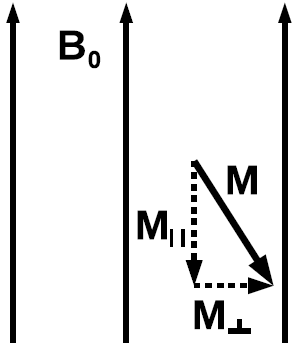
\includegraphics[width=30mm]{./Resources/magnetization_components.png}
	\caption{Zerlegung der Magnetisierung in Komponenten}
\end{figure}

Im Grundzustand ist die Magnetisierung parallel zu den Feldlinien, in angeregten Zuständen können wir diese in einen Anteil $M_{\perp}$ senkrecht und $M_{\parallel}$ parallel zu den Feldlinien aufspalten. Angeregte Zustände zerfallen dabei auf einer charakteristischen Zeitskala in den Grundzustand.
\begin{figure}[!htb]
	\centering
	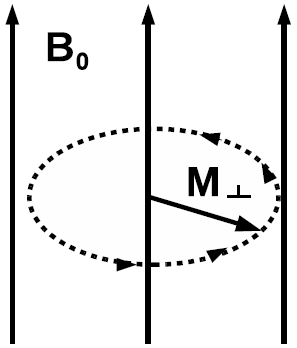
\includegraphics[width=30mm]{./Resources/larmor_precession.png}
	\caption{Larmor-Präzession von $M_{\perp}$}
\end{figure}

Die Wechselwirkung zwischen dem Magnetfeld $\vec{B_0}$ und der Magnetisierung $\vec{M}$ führt zu einem Drehmoment $\vec{\tau}$, wodurch $M_{\perp}$ mit einer Winkelfrequenz $\omega_{L}$ um $\vec{B_0}$ präzediert. Diese sogenannte Larmorfrequenz ist gegeben durch:
\begin{equation}
\omega_{L} = \gamma B_0
\end{equation}
\begin{figure}[!htb]
	\centering
	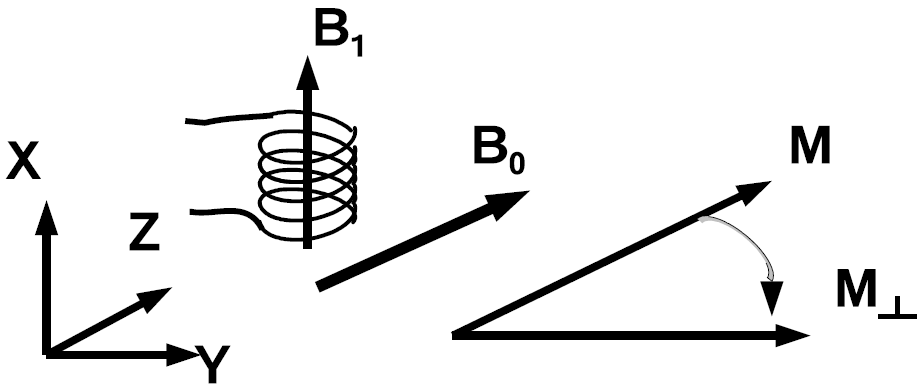
\includegraphics[width=70mm]{./Resources/hf_pulse.png}
	\caption{Hochfrequenzpuls zur Rotation der Magnetisierung}
\end{figure}
Eine bestimmte Magnetisierung kann durch Anlegen eines HF-Pulses an die Magnetisierung im Grundzustand erzeugt werden. Das zusätzliche Magnetfeld $\vec{B_1}$ dreht die Grundzustandsmagnetisierung während eines Zeitintervalls $\Delta t$ um einen Winkel
\begin{equation}
\alpha = \gamma B_1 \Delta t
\end{equation}
Ist die Zeitdauer so gewählt, dass $\alpha = 90^\circ$, wird $\vec{M}$ in eine senkrechte Komponente $M_{\perp}$ überführt ($90^\circ$-Puls). Ebenfalls kann durch $\alpha = 180^\circ$ eine Magnetisierung antiparallel zu dem statischen Feld $\vec{B_0}$ erzeugt werden ($180^\circ$-Puls).

\subsection{Kalibration des Systems}

An der Spule, auf die der HF-Puls gegeben wird, kann ebenfalls eine durch die präzedierende Magnetisierung hervorgerufene Induktionsspannung gemessen werden. Da dieses Signal mit der Larmorfrequenz $\omega_L$ moduliert ist, liefert eine Fouriertransformation Aufschluss über die Frequenzverteilung der Probe.
\newline\newline
Zunächst müssen die im Gerät als \texttt{PULS I} und \texttt{PULS II} ausgezeichneten Signalformen über die Pulsdauer als $90^\circ$- bzw $180^\circ$-Puls definiert werden. In Abbildung \ref{fig:pulse_signal} ist die Form eines solchen Pulses direkt nach dem Signalgenerator zu erkennen. Über die Potentiometer S6 und S7 ist die zeitliche Länge variierbar.

Um nun die Pulse zu kalibrieren, wird das in der Spule induzierte Signal auf dem Oszilloskop beobachtet (s. Abb. \ref{fig:pulse_induced}). \texttt{PULS I} entspricht genau dann einer Drehung um $90^\circ$, wenn die Anstiegsflanke des Pulses maximal steil ist, \texttt{PULS II} einer Drehung um $180^\circ$, wenn die Flanke möglichst flach ist.
\newline
\begin{figure}[!htb]
	\centering
	% hier schon der komplixiert Fall, dass 2 Bilder nebeneinander gesetzt werden
	\parbox{60mm}{
		\centering
		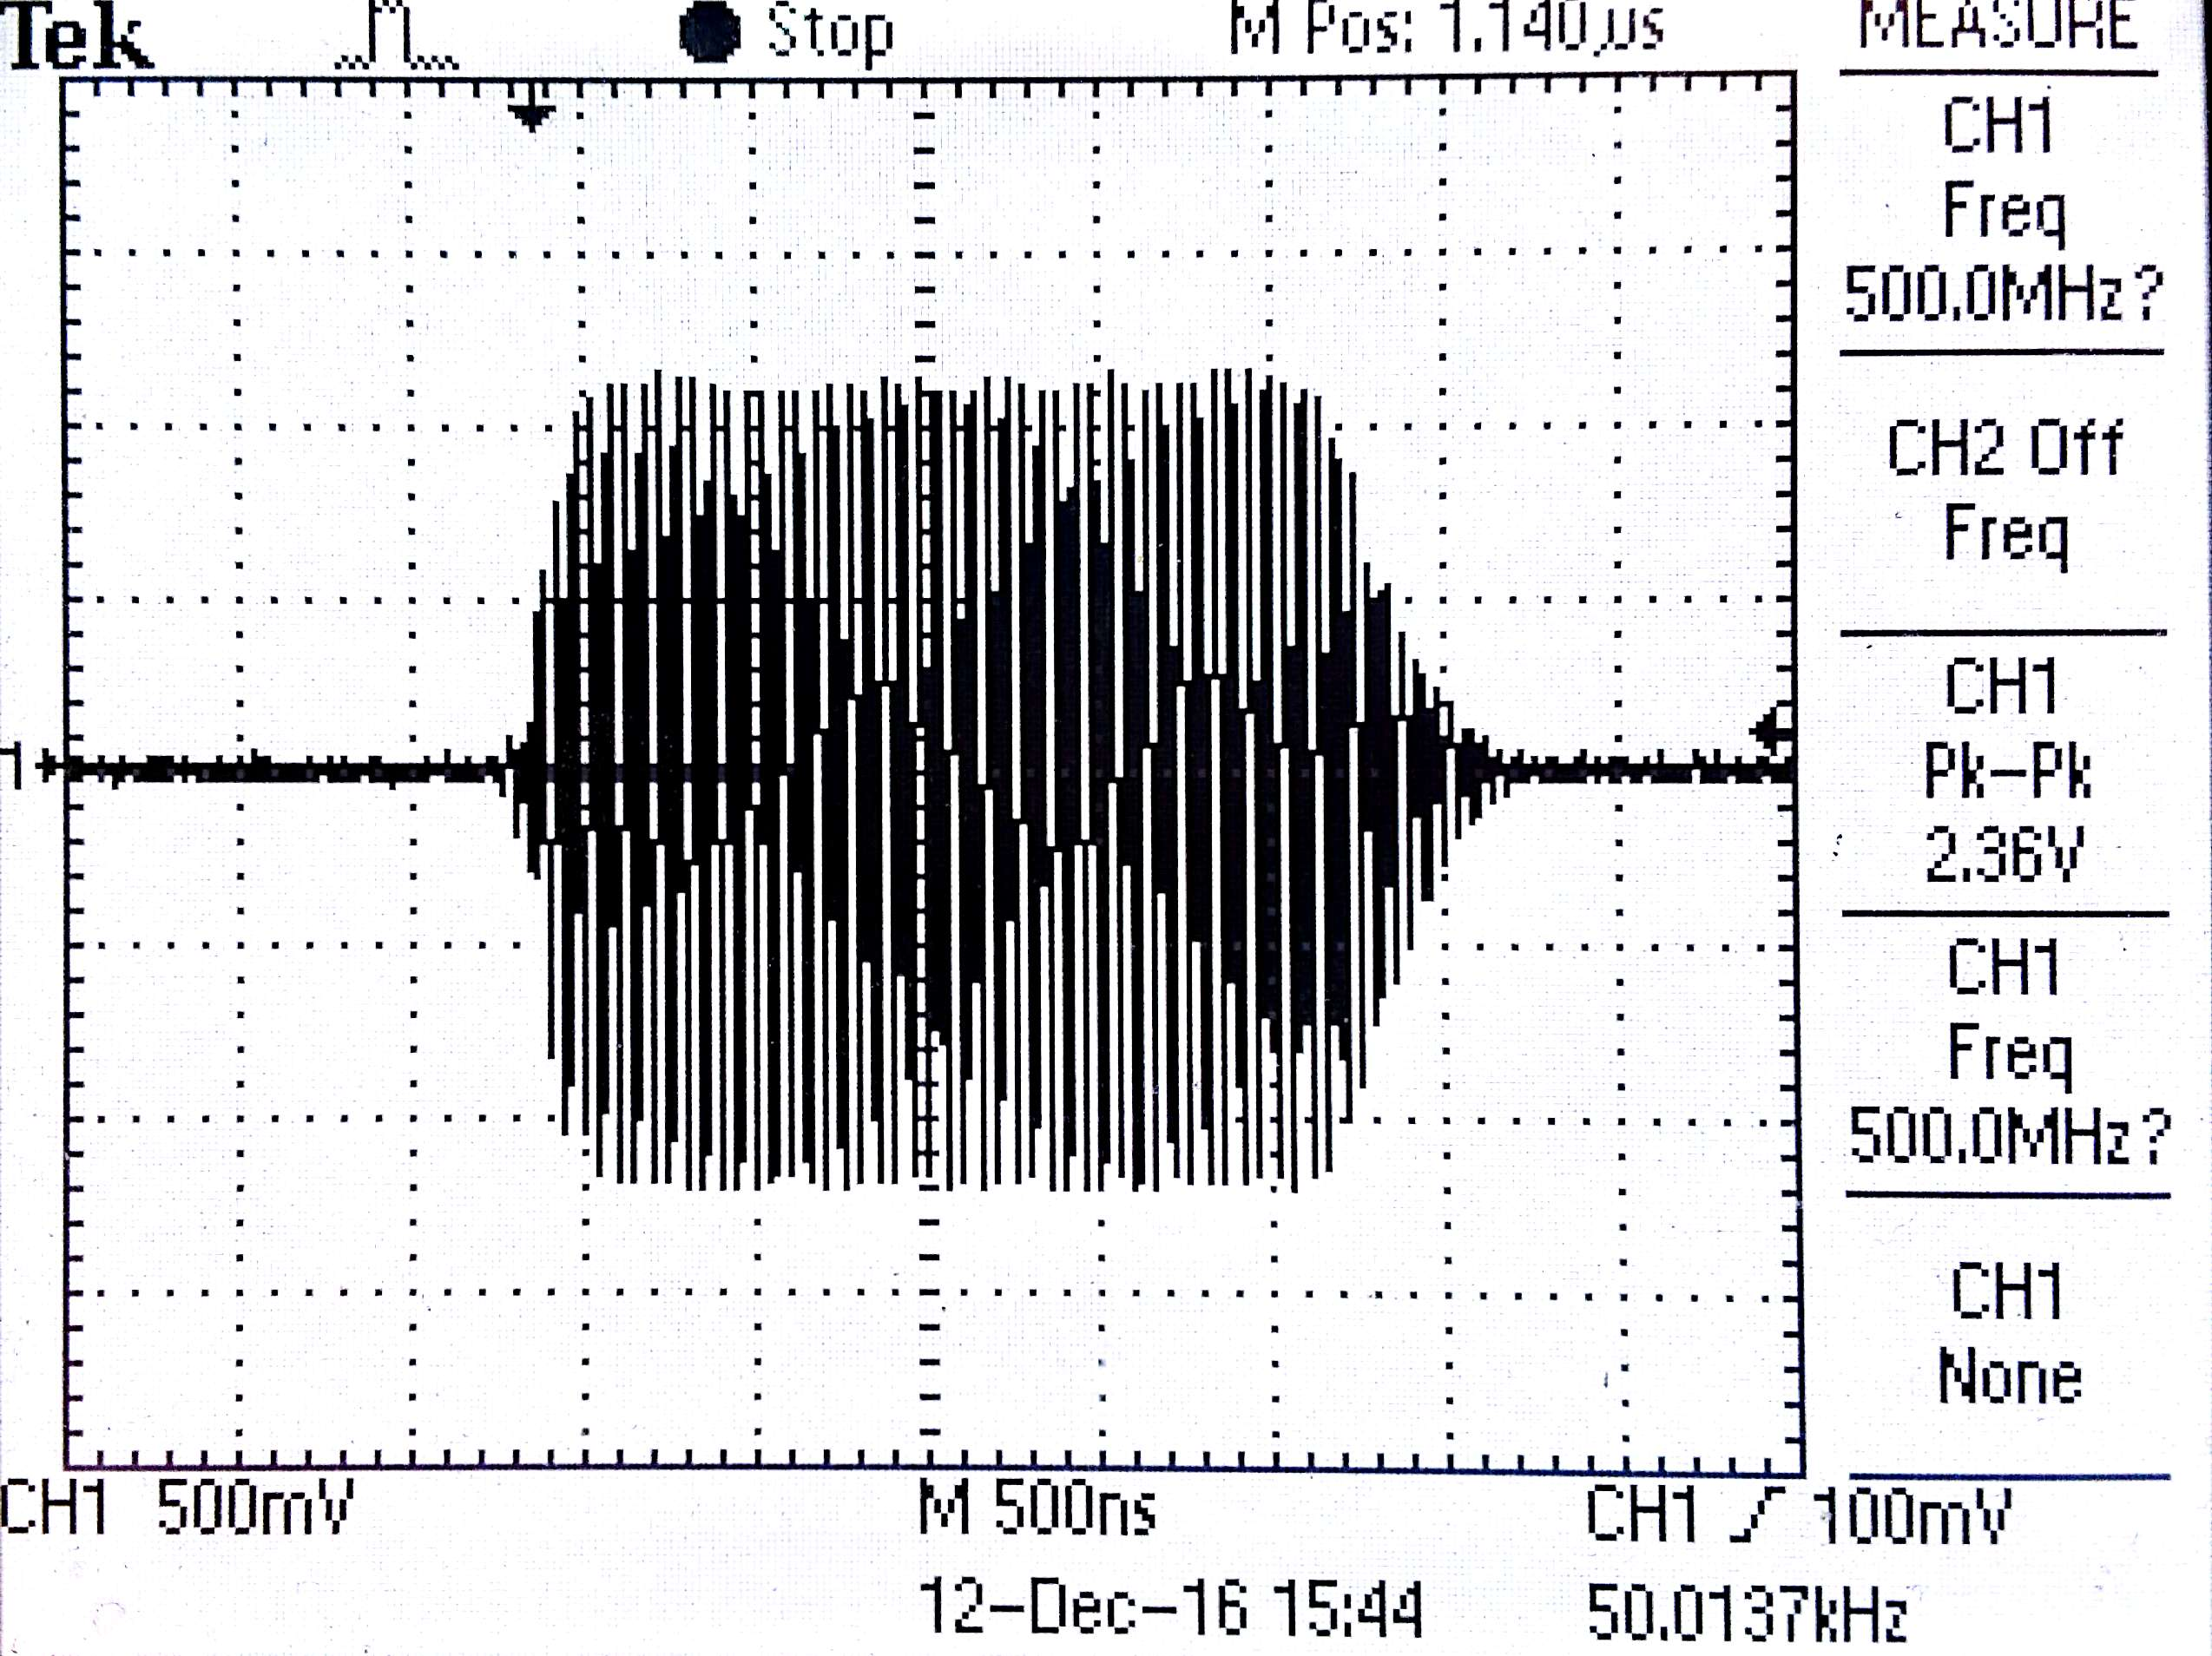
\includegraphics[width=55mm]{./Resources/pulse_train.jpg}
		\caption{Pulsform direkt nach dem Signalgenerator.}
		\label{fig:pulse_signal}
	}
	\hfill  % fuegt Platz ein, das rueckt die beiden Bilder an den Rand
	\parbox{60mm}{
		\centering
		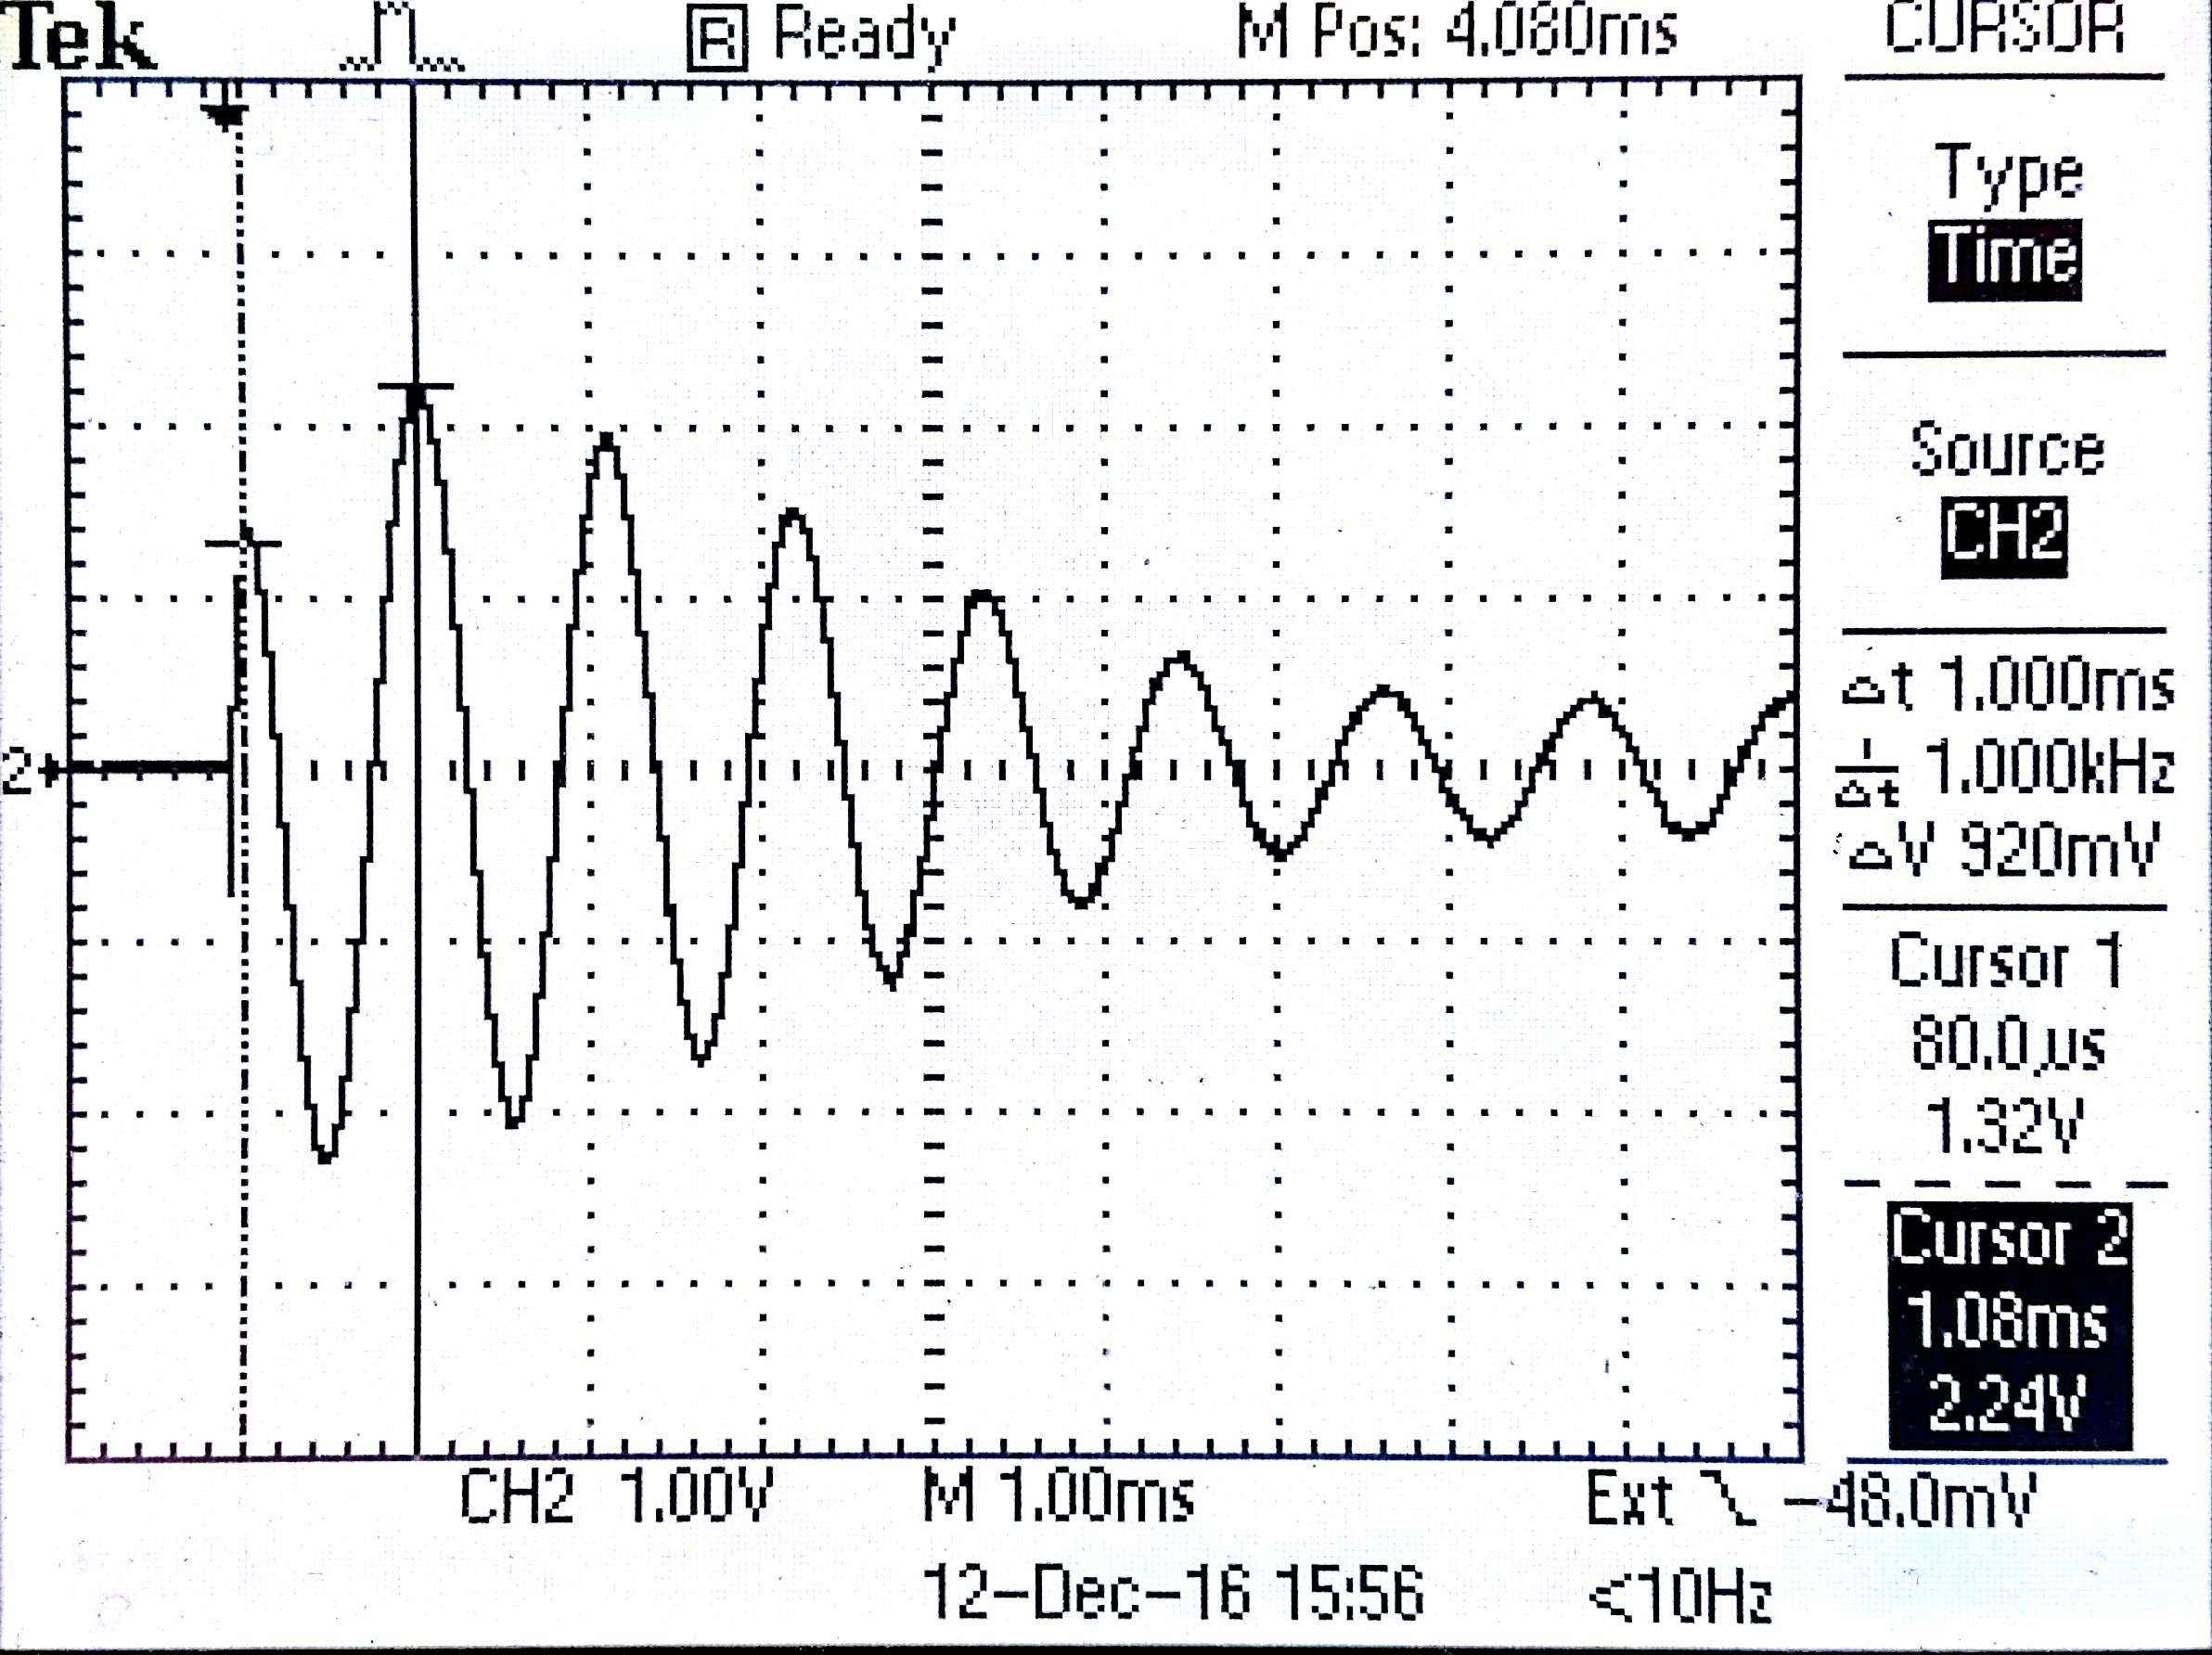
\includegraphics[width=55mm]{./Resources/single_pulse_event.jpg}
		\caption{Induziertes Signal in der Spule zur Pulskalibration.}
		\label{fig:pulse_induced}
	}
\end{figure}

Für die Kalibration wird Probe I (Gd 1:500 in Wasser) verwendet. Die HF-Pulse sind jeweils mit einer Frequenz von $\omega_{HF} = (19.9 \pm 0.2) MHz$ moduliert. Die Arbeitsfrequenz wird nun durch Drehen der Schraube W1 auf $1kHz$ eingestellt. \texttt{PULS I} hat dann $90^\circ$-Verhalten, wenn $S6 \approx 2.0$ (Amplitude ca. $6V$), \texttt{PULS II} $180^\circ$-Verhalten, wenn $S7 \approx 2.1$ (Amplitude ca. $7V$). Über die FWHM des Pulses bestimmen wir die Pulsbreite zu:
\begin{itemize}
	\item[] \texttt{PULS I}: $t_1=\err{1,41}{0,10}\us$
	\item[] \texttt{PULS II}: $t_2=\err{2,48}{0,20}\us$
\end{itemize}

\section{Durchführung und Auswertung}

\subsection{Teil I: Relaxationszeiten}

\subsubsection{Theorie}

Relaxiert eine angeregte Magnetisierung zurück in den Grundzustand, so kann deren zeitliche Entwicklung durch die Bloch-Gleichungen beschrieben werden. In einem mitbewegten Bezugssystem sind diese gegeben durch:

\begin{equation}
\frac{dM_{\perp}(t)}{dt} = - \frac{M_{\perp}(t)}{T2}
\end{equation}
\begin{equation}
\frac{dM_{\parallel}(t)}{dt} = - \frac{M_{\parallel}(t) - M_0}{T1}
\end{equation}

Zu der Energie eines angeregten Zustands tragen ma"sgeblich zwei verschiedene Wechselwirkungen bei. Der erste Anteil ist gegeben durch die Wechselwirkung der magnetischen Dipole mit dem externen Feld (Spin-Gitter Wechselwirkung). Zweitens interagieren auch die einzelnen Dipolmomente untereinander, wobei eine antiparallele Orientierung energetisch günstiger ist (Spin-Spin Wechselwirkung).

Die zeitliche Entwicklung einer transversalen Magnetisierung ergibt sich aus der Lösung von Gl. (4) zu:

\begin{equation}
M_{\perp}(t) = M_{\perp}^0 e^{-\frac{t}{T_2}}
\end{equation}

Die Spin-Spin Relaxationszeit $T_2$ kann durch die sogenannte Spin-Echo Methode bestimmt werden.
\newline
\begin{figure}[!htb]
	\centering
	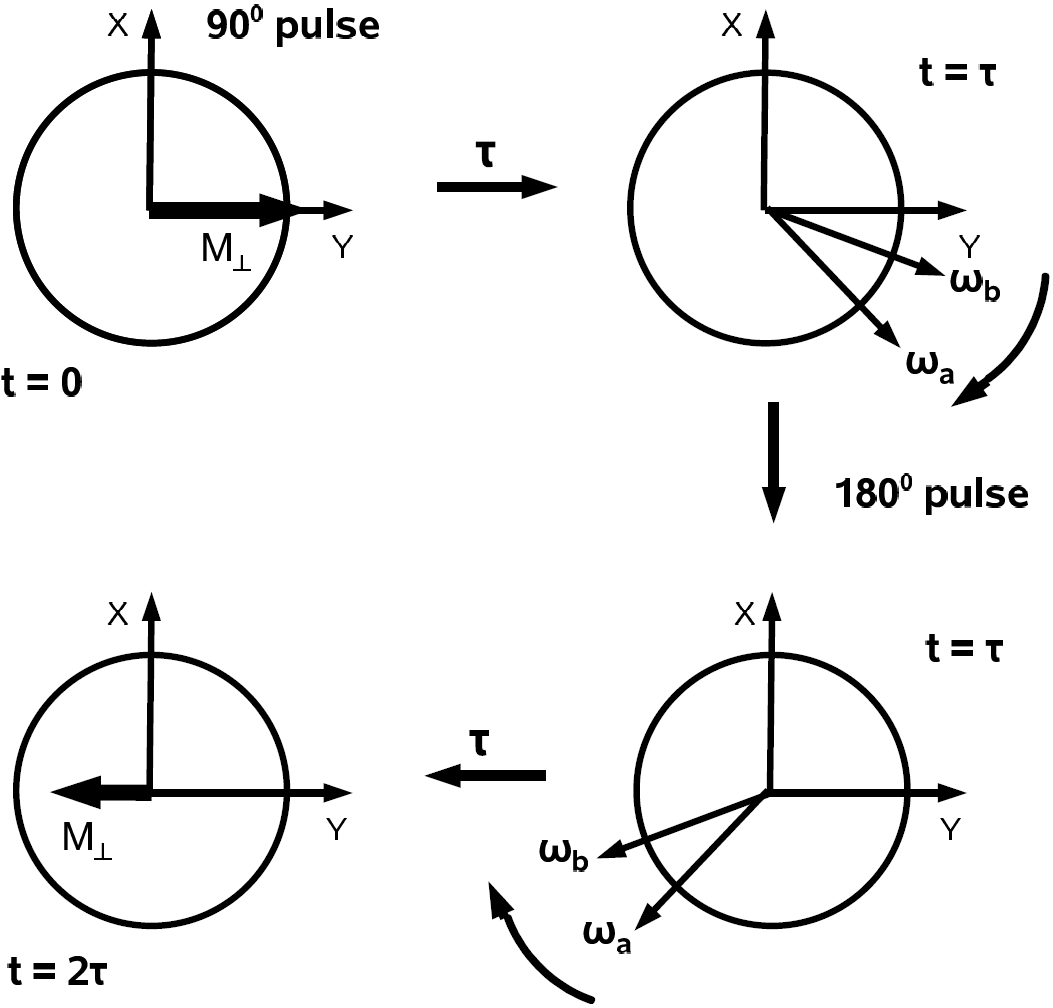
\includegraphics[width=80mm]{./Resources/spin_ech_schematic.png}
	\caption{Prinzip der Spin-Echo Methode}
	\label{fig:spinecho_bloch}
\end{figure}

Hierbei wird zunächst mit einem $90^\circ$-Puls eine transversale Magnetisierung erzeugt. Aufgrund des Magnetfelds $\vec{B_0}$ präzediert die Magnetisierung dann, wobei Protonen an unterschiedlichen aufgrund von Inhomogenitäten des Magnetfelds unterschiedliche Larmorfrequenzen haben. Zwei unterschiedliche Protonen haben dann zum Zeitpunkt $t=\tau$ eine Phasendifferenz aufgebaut, die durch Gabe eines $180^\circ$-Pulses umgekehrt werden kann. Nach der Zeit $t=2\tau$ sind die Magnetisierungen wieder in Phase, und das so erzeugte 'Spin-Echo' kann auf dem Oszilloskop beobachtet werden (s. Abb. \ref{fig:spinecho_osci}).
\newline
\begin{figure}[!htb]
	\centering
	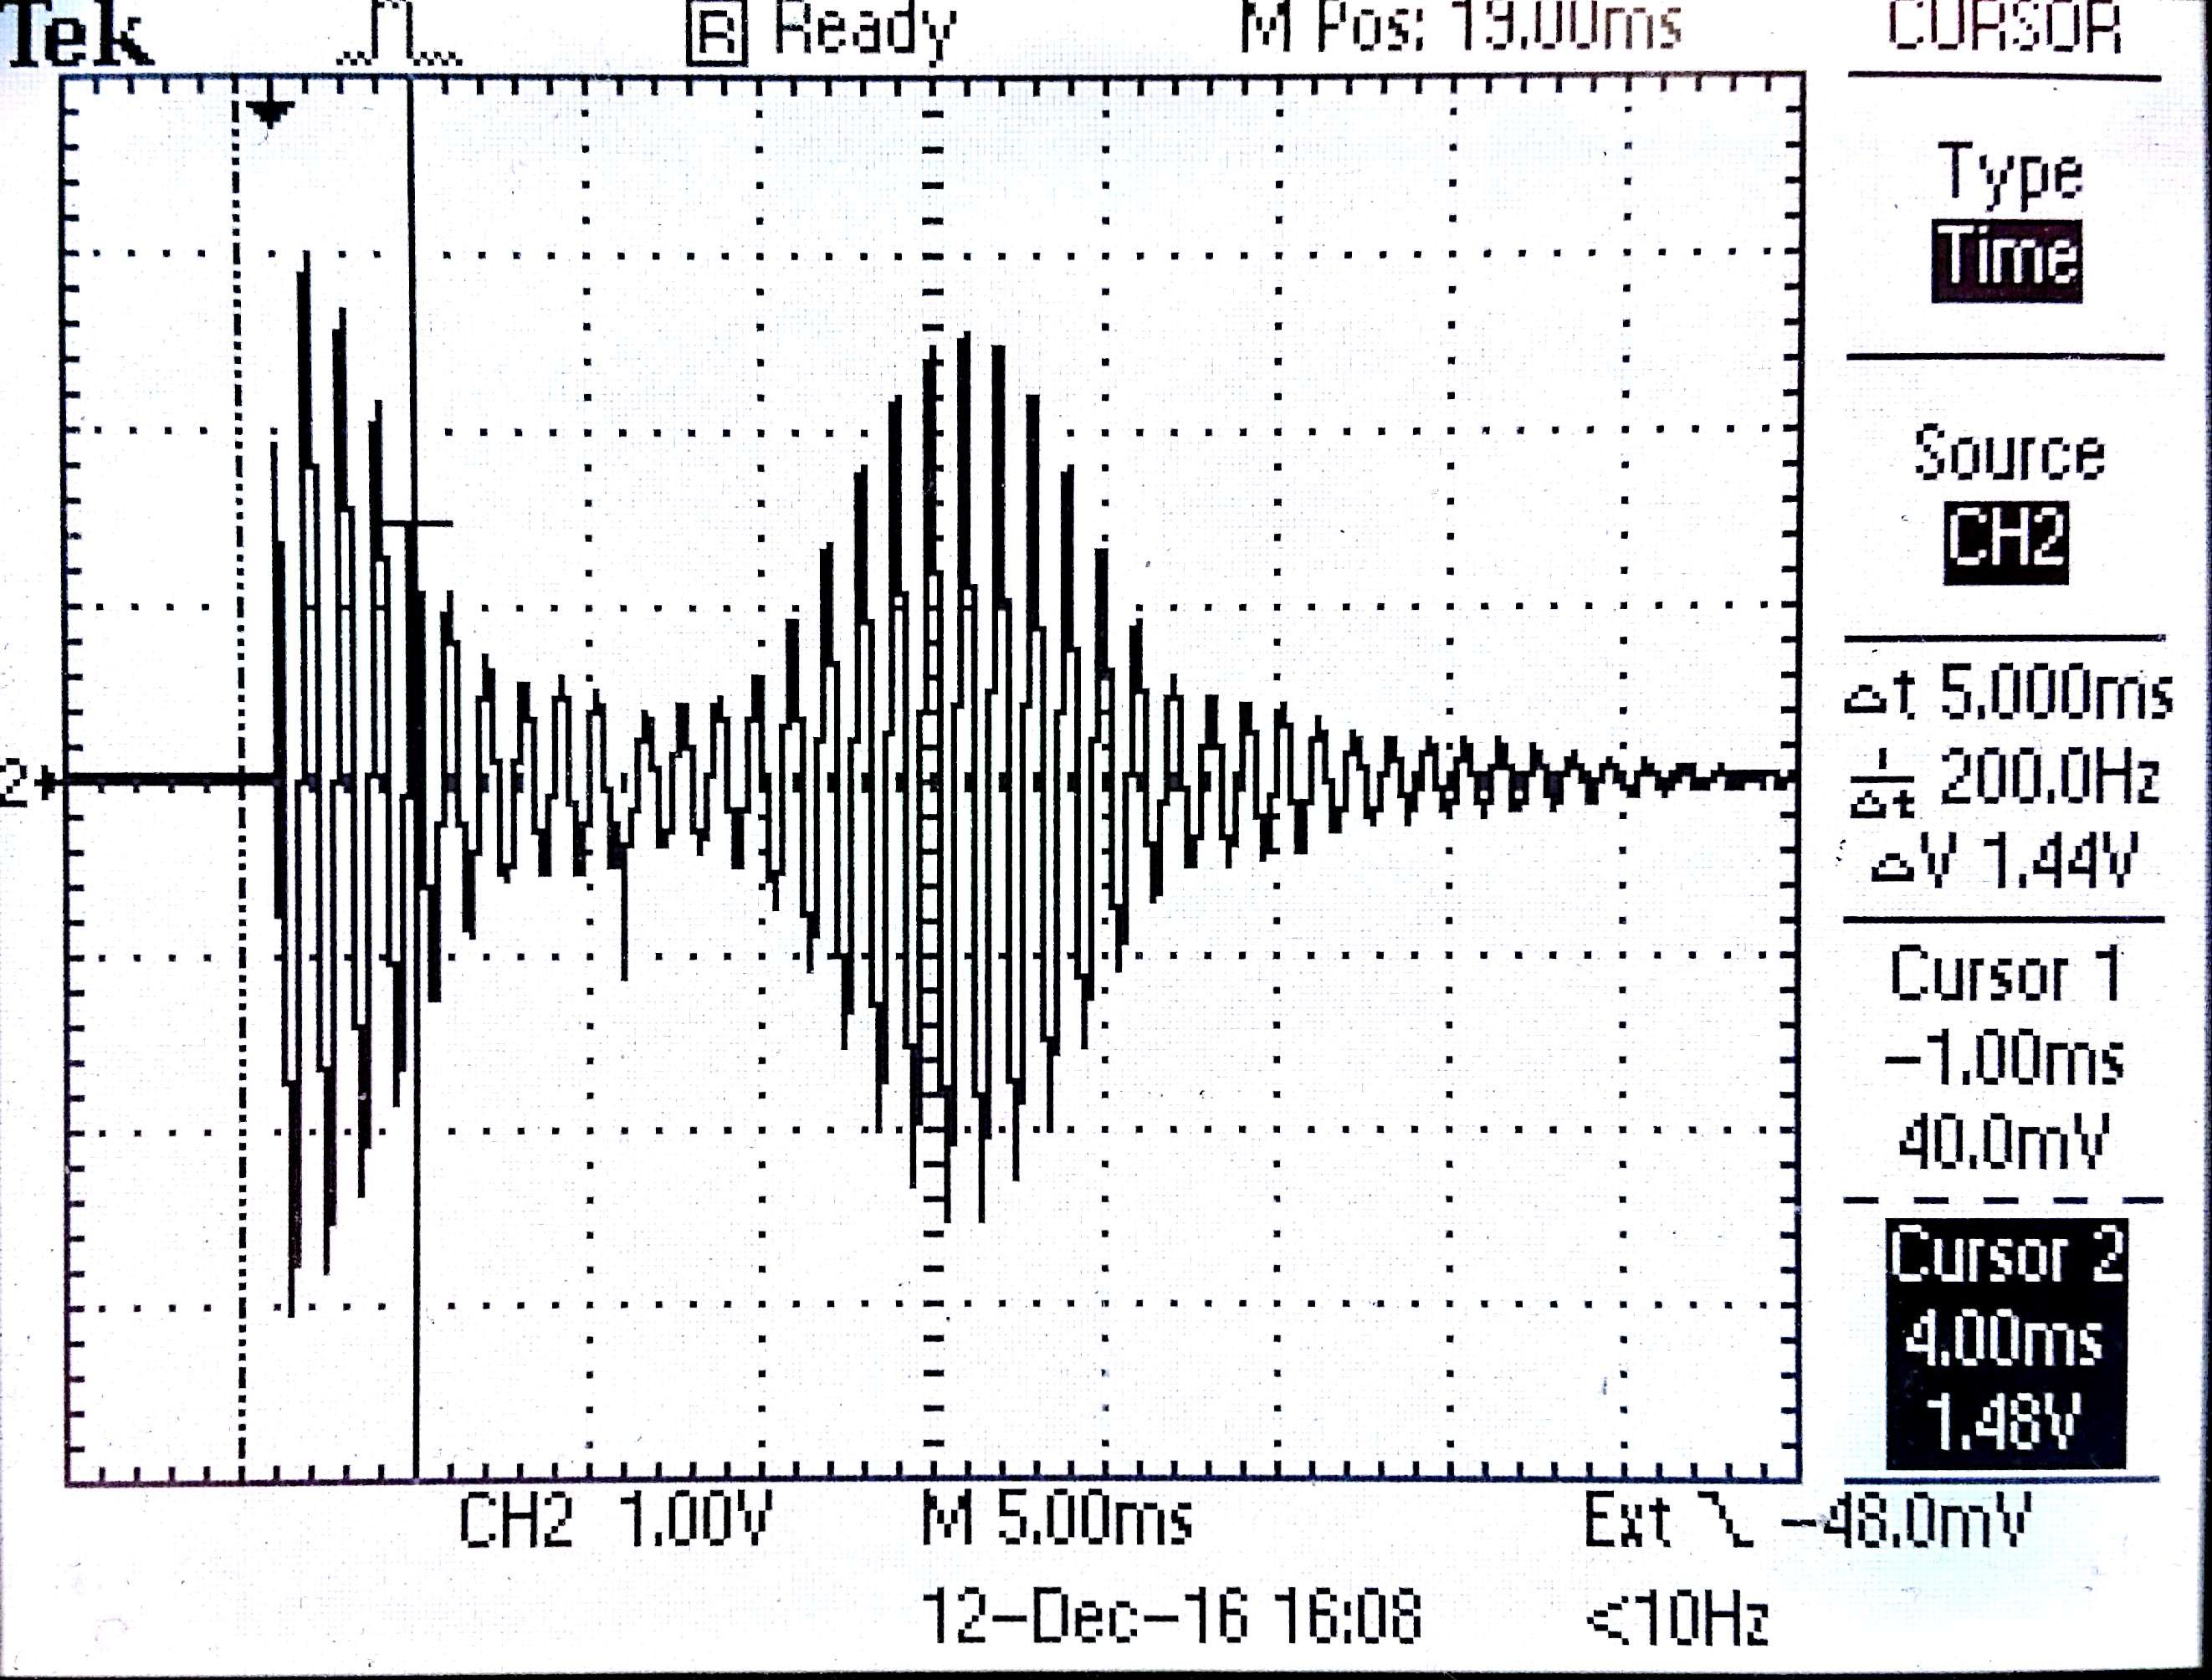
\includegraphics[width=80mm]{./Resources/spinecho_osci.jpg}
	\caption{Spin-Echo Messung mit $\tau=10ms$}
	\label{fig:spinecho_osci}
\end{figure}

Durch Messung des Maximums der Einhüllenden zu verschiedenen Zeiten $\tau$ können also Punkte des Zerfallsgesetztes in Gl. (6) aufgenommen werden. 
Die Spin-Echo Methode wird für lange Zeiten zunehmend ungenau, da die Protonen vor Anlegen des $180^\circ$-Pulses an andere Positionen diffundieren können. Hierdurch kann nur teilweise Kohärenz erreicht werden; das Signal wird kleiner und wir messen zu niedrige Werte für $T_2$.
\newline\newline
Diese Limitation kann durch Verwendung einer sogenannten Carr-Purcell Sequenz minimiert werden. Hierbei wird wie gehabt mit einem $90^\circ$-Puls gestartet, und nach allen ungeraden Vielfachen einer kurzen Zeit $\tau$ wird ein $180^\circ$-Puls angelegt. Zu allen geraden Vielfachen von $\tau$ ist das System phasenkohärent, und wir können die Relaxation der Magnetisierung mit einer höheren Genauigkeit messen.
\newline\newline
Die zeitliche Entwicklung einer antiparallelen Magnetisierung ergibt sich aus der Lösung von Gl. (5) zu:
\begin{equation}
M_{\parallel}(t) = M_{\parallel}^0(1-2e^{-\frac{t}{T_1}})
\end{equation}
Die Spin-Gitter Relaxationszeit $T1$ kann bestimmt werden, in dem zunächst mit eine, $180^\circ$-Puls gestartet wird. Diese Magnetisierung produziert kein Signal, weshalb nach einer Zeit $t=\tau$ ein $90^\circ$-Puls zur Messung angelegt werden muss. Ähnlich der Spin-Echo Methode können nun unterschiedliche Punkte der Zerfallskurve durch Messung bei variablen Werten von $\tau$ bestimmt werden.

\subsubsection{Durchführung}

Zunächst wird mithilfe der Spin-Echo Methode die Relaxationszeit $T2$ bestimmt.

\newpage

\subsection{Teil II: Chemische Verschiebung}

\subsubsection{Theorie}

\newpage

\subsubsection{Durchführung}

\newpage

\subsection{Teil III: Bildgebung mit NMR}

\subsubsection{Theorie}

\newpage

\subsubsection{Durchführung}

\newpage

\section{Zusammenfassung und Fazit}


\end{document}